\documentclass[letterpaper,11pt]{article}

% Soporte para los acentos.
\usepackage[utf8]{inputenc}
\usepackage[T1]{fontenc}    
% Idioma español.
\usepackage[spanish,mexico, es-tabla]{babel}
% Soporte de símbolos adicionales (matemáticas)
\usepackage{multirow}
\usepackage{amsmath}
\usepackage{amssymb}
\usepackage{amsthm}
\usepackage{amsfonts}
\usepackage{mathtools}
\usepackage{latexsym}
\usepackage{enumerate}
\usepackage{ragged2e}
\usepackage{graphicx}
\usepackage{hyperref}
\usepackage{xcolor}
% Modificamos los márgenes del documento.
\usepackage[lmargin=1cm,rmargin=1cm,top=1.5cm,bottom=1.5cm]{geometry}

\title{Facultad de Ciencias, UNAM \\ 
       Lenguajes de Programación \\ 
       Tarea 3}
\author{Hernández Salinas Óscar \\ 
        Rubí Rojas Tania Michelle }
\date{26 de octubre de 2020}

\begin{document}
\maketitle

\begin{enumerate}
   % Ejercicio 1.
   \item Evalúa las siguientes expresiones usando \texttt{a) alcance estático}
   y \texttt{b) alcance dinámico}. Es necesario que muestres el ambiente de 
   evaluación final en forma de pila y en forma de lista en cada caso.
   \begin{enumerate}
       % Ejercicio 1.a
       \item 
       \begin{verbatim}
       {with {a 2} 
          {with {b 3} 
             {with {foo {fun {x} {- {+ a b} x}}} 
                {with {a -2} 
                   {with {b -3} 
                      {with {foo {fun {x} {+ {- a b} x}}} 
                         {foo -10}}}}}}}
       \end{verbatim}

       \textsc{Solución:}

       % Ejercicio 1.b
       \item 
       \begin{verbatim}
       {with {foo {fun {x} {+ x {foo {- x 1}}}}} 
          {foo 10}}
       \end{verbatim}

       \textsc{Solución:}

       % Ejercicio 1.c
       \item 
       \begin{verbatim}
       {with {x 2} 
          {with {foo {fun {a} {+ x 2}}} 
             {with {y 3} 
                {with {foo {fun {b} {- y b}}} 
                   {with {x 4} 
                      {with {goo {fun {b} {+ {foo x} {foo y}}}} {goo 3}}}}}}}
       \end{verbatim}

       \textsc{Solución:}
   \end{enumerate}

   % Ejercicio 2.
   \item Las primeras versiones del lenguaje \textsc{Lisp} hacían uso de 
   alcance dinámico y sus diseñadores se negaban a cambiárlo debido a una 
   gran ventaja que traía consigo el uso de este tipo de alcance. Con base 
   en los resultados obtenidos en el inciso \texttt{(b)} del ejercicio 
   anterior, menciona esta ventaja.

   \textsc{Solución:}

   % Ejercicio 3.
   \item En clase se revisó que la función de \textit{sustitución} es 
   ineficiente, ya que en el peor caso es de orden cuadrático en relación 
   al tamaño del programa (considerando el tamaño del programa como el 
   número de nodos en el árbol de sintaxis abstracta). Por otro lado, se 
   expuso una alternativa a este algoritmo de sustitución usando 
   ambientes. Sin embargo, el implementar un ambiente usando una pila no 
   parece ser mucho más eficiente.
   \begin{enumerate}
        % Ejercicio 3.a
        \item Da un programa que ilustre la no linealidad de la implementación
        basada en pilas y explica brevemente por qué su ejecución en tiempo no
        es lineal con respecto al tamaño de la entrada.

        \textsc{Solución:} Supongamos que tenemos el siguiente programa, el 
        cual tiene $n$ variables de-ligado.
        \begin{verbatim}
        {with {x 1} 
           {with {a_1 x} 
              {with {a_2 x} 
              ...
                 {with {a_{n-1} x}} 
                    {+ x {+ a_1 {+ a_2 + {+ ... {+ a_{n-1} x} ... }}}}}}}
        \end{verbatim}

        \begin{figure}[h]
            \centering
            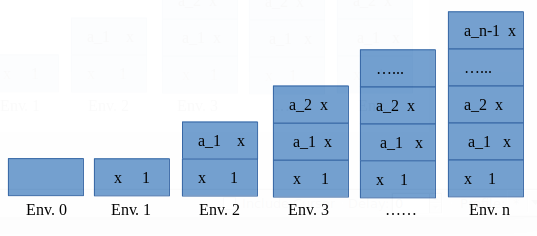
\includegraphics[width=0.5\linewidth]{imagenes/ejercicio3.png}
            \caption{Ambiente en forma de pila}
        \end{figure}

        Notemos que a cada una de las variables de ligado le corresponde una 
        variable ligada. Entonces, la primer variable que nos encontramos es
        $x$, así que buscamos esta variable en nuestro ambiente (que está al 
        fondo de la pila). La siguiente variable que nos encontramos es 
        \texttt{$a_1$}, pero el valor que le corresponde es aquel que posee 
        $x$, por lo que tenemos que volver a buscar dentro del ambiente 
        para poder asignarle un valor a nuestra variable \texttt{$a_1$}. 
        De manera análoga, las demás variables $a_i$ tendrán que realizar el 
        mismo procedimiento para poder asignarle el valor a su variable. 
        Por lo que, cada una de las $n$ variables tiene que buscar el valor 
        de $x$ en el ambiente. Esto nos toma tiempo $O(n^2)$ ya que buscar 
        un elemento en la pila, en el peor caso, es lineal; pero estamos 
        aplicándo esto a cada una de las $n$ variables que tiene nuestro 
        programa, lo que justifica nuestra complejidad cuadrática. 

        % Ejercicio 3.b
        \item Describe una estructura de datos para un ambiente que un 
        intérprete de FWAE pueda usar para mejorar su complejidad. Muestra 
        cómo el intérprete usaría esta nueva estructura de datos. Indica 
        además, cuál es la nueva complejidad del intérprete (análisis del 
        peor caso).

        \textsc{Solución:} Los diccionarios (o \textit{hash tables}) son 
        estructuras de datos que nos ayudan a asociar llaves con valores. 
        La operación principal que soporta de manera eficiente es la 
        búsqueda, ya que permite el acceso a los elementos almacenados a partir 
        de una llave generada. Funciona transformando la llave con una 
        \textit{función hash} en un hash, un número que identifica la posición 
        donde la tabla hash localiza el valor deseado. 

        Los diccionarios se suelen implementar sobre arreglos, por lo que proveen
        tiempo constante de búsqueda, sin importar el número de elementos en la
        tabla. Sin embargo, en casos particularmente malos, el tiempo de búsqueda 
        puede llegar a ser lineal.

        Así pues, nuestra propuesta es utilizar un diccionario como estructura 
        de datos, ya que el código hash de cada una de las variables es su 
        propia llave y su valor, lo que nos permitirá poder buscar en el 
        ambiente el valor de las variables. Por lo que, si la primer variable 
        ligada que nos encontramos es $x$ (con un valor de $1$), entonces 
        podemos agregar esta información al diccionario (nuestro ambiente) y 
        aplicar esto a cada una de las variables que vayamos encontrando.

        Así, cada vez que mandemos a llamar una función, nos tomará tiempo 
        constante (salvo casos particularmente malos) tomar el valor del último 
        ambiente y ponerlo en nuestra función. En el peor caso, la función que 
        mandamos a llamar carga con todas las variables que tenemos hasta el 
        momento, lo que hará que nos tome tiempo lineal (con respecto al número 
        de elementos en la \textit{tabla hash}).

   \end{enumerate}
\end{enumerate}

\begin{thebibliography}{2}
  \bibitem{1}
  Hash tables \\
  \url{https://en.wikipedia.org/wiki/Hash_table}
\end{thebibliography}

\end{document}
